\chapter{Grundlagen}
\label{chap:Grundlagen}

\todo{Quellen}
	\section{Stacked Convolutional Autoencoder }
	\label{sec:StackedConvolutionalAutoencoder}		
	
	\todo{sec:StackedConvolutionalAutoencoder }
			\begin{figure}[h]
				\centering
				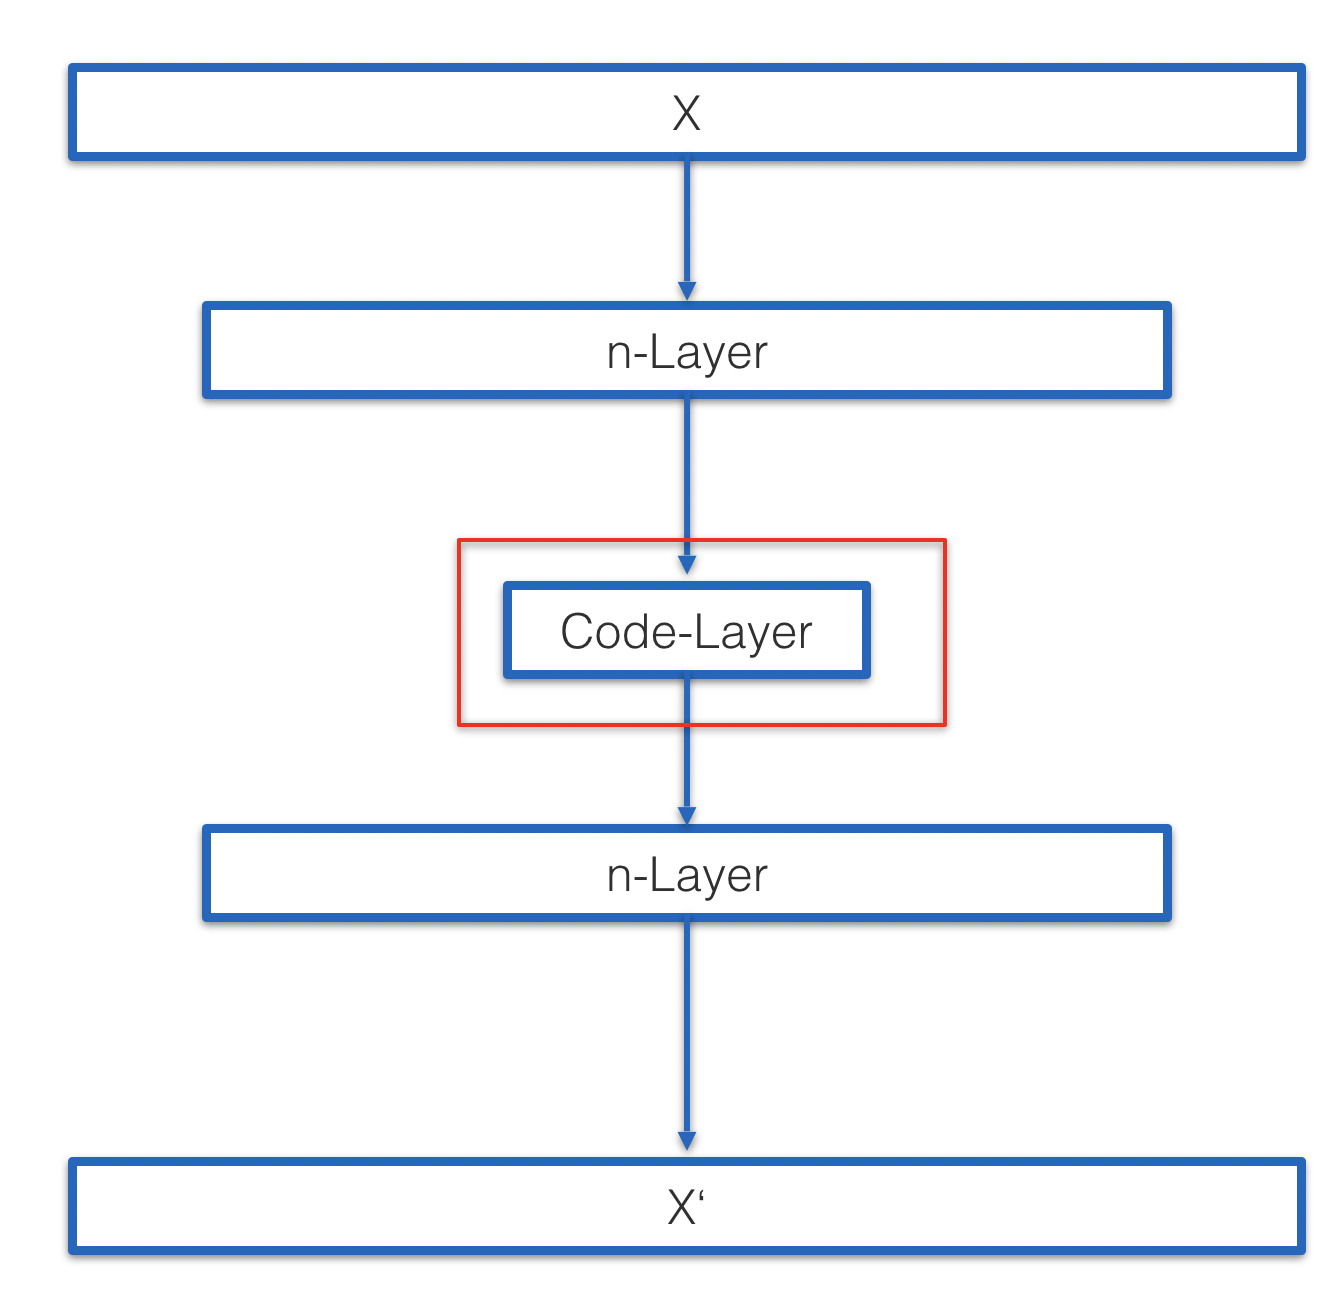
\includegraphics[width=0.5\textwidth, center]{bilder/Schema_Autoencoders/Schema_CAE.png}
				\caption[Schema Autoencoder]{Schema Autoencoder}
				\label{img:SchemaCAE}
			\end{figure}  

		\subsection{Layerwise Pretrain }

		Warum pretrian?:	https://papers.nips.cc/paper/3048-greedy-layer-wise-training-of-deep-networks.pdf (Warum machen das andere heute nicht mehr? viele cnn haben vanishing gradients problem  über relu,... gelösst) (weitere literatur: möglicherweise Geoffrey E. Hinton)

		Stacked Convolutional Auto-Encoders Stacked Convolutional Auto-Encoders for
		Hierarchical Feature Extraction
		Jonathan Masci, Ueli Meier, Dan Ciresan, and Jurgen Schmidhuber
		Istituto Dalle Molle di Studi sullIntelligenza Artificiale (IDSIA)
		Lugano, Switzerland
		{jonathan,ueli,dan,juergen}@idsia.ch
		
		- layerwise pretrain {Greedy Layer-Wise Training of Deep Networks}

	\section{ Transferlernen}
	\label{sec:Transferlernen}
		\todo{sec:Transferlernen }
		- Was ist das
		-	oberste Schichten allgemeiner als untere --> todo papaer verweisen
	\section{AutoML}
	\label{sec:AutoML}
			\todo{AutoML }
		Was ist das
		\subsection{RandomSearch}
		
		\subsection{HyperBand }

		\subsection{BOHB }


	\section{Bibliotheken und Werkzeuge}
	\label{sec:BibliothekenundWerkzeuge}
	Für den praktischen Teil der Abschlussarbeit wurde insbesondere Cnvrg \cite{cnvrg.io.} genutzt. Cnvrg.io ist eine "full-stack Data Science Platform" welche Werkzeuge für die Erstellung, Verwaltung, Bereitstellung und Automatisierung von maschinellem Lernen bereitstellt. Cnvrg erlaubt es Arbeitsbereiche mittels Containern zu erstellen. Die Container können dabei auf Maschinen in Azure \cite{Micorsoft.2020} zugreifen. Für die Experimente wurde ein vorgefertigter Container mit einer tesla-k80 \cite{Nvidia.2020}, fünf CPUs und 49 GB Arbeitsspeicher genutzt. 

	Für die Entwicklung wurden Python \cite{PythonSoftwareFoundation.2020}, Jupyter Notebooks \cite{ProjectJupyter} und das Framework Tensorflow \cite{MartinAbadi.2015}  genutzt. Die wichtigsten Bibliotheken für die Arbeit sind Keras \cite{Chollet.2015} , Numpy \cite{Oliphant.2006} , Matplotlib \cite{Hunter.2007} , scikit-learn \cite{Pedregosa.2011} , ConfigSpace \cite{Lindauer.8162019} , Bayesian Optimization and Hyperband \cite{StefanFalkner.2018}. 
	
	Für die Visualisierung von Bildeinbettung wurde das Werkzeug "PSIORI Visualizer" erweitert und eingesetzt. Der Visualizer erlaubt es Daten in 3-D darzustellen. Dabei können Filter eingesetzt werden, der Blickwinkel geändert werden, die Daten mit zusätzlicher Information versehen werden und Zoomen ist möglich.
	
	\begin{figure}[h]
		\centering
		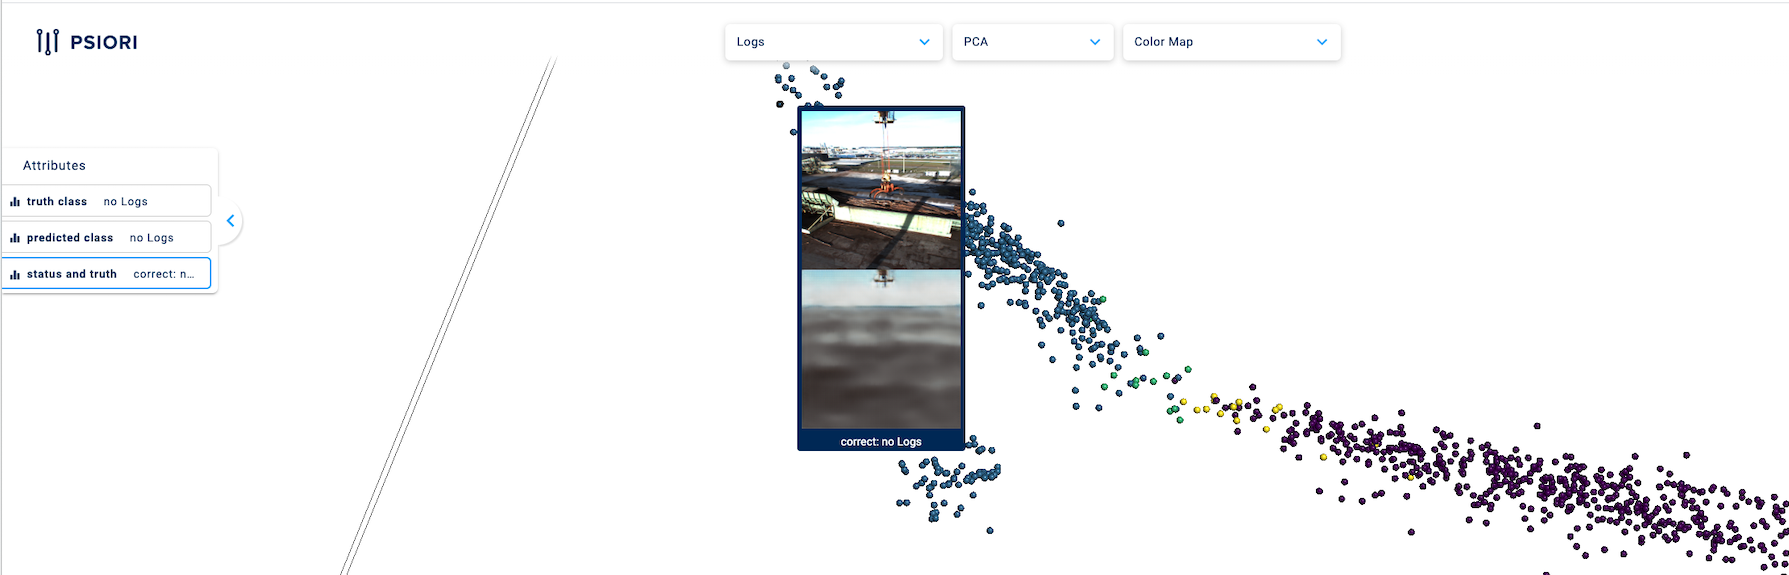
\includegraphics[width=1\textwidth, center]{bilder/Grundlagen/Example_Visualizer.png}
		\caption[Beispiel PSIORI Visualizer]{Beispiel PSIORI Visualizer}
		\label{img:ExampleVisualizer}
	\end{figure}  
	Die Abbildung \ref{img:ExampleVisualizer} zeigt einen Screenshot einer Visualisierung einer Einbettung. Als zusätzliche Information sind die Datenpunkte entsprechend einer Klassifikation in True-Positiv, True-Negativ, False-Negativ und False-Positiv eingefärbt. Wird über einen Datenpunkt mit der Maus geschwebt, werden zusätzliche Informationen zu dem Datenpunkt angezeigt. Diese Funktion wurde insbesondere zum Anzeigen eines Originalbildes, ihrer Rekonstruktion mittels Autoencoder und einer Beschriftung genutzt. 
	
	Kern der erstellten Werkzeuge ist das Framework  Psipy \cite{PSIORIGmbH.2019}. Psipy ist ein Python-Framework für maschinelles Lernen welches von PSIORI selbst entwickelte Modelle zusammenfasst und eine einheitliche API zu Verfügung stellt. Diese API ist an die API des verbreiteten Frameworks scikit-learn angelehnt. Es können Modelle basierend auf scikit-learn  und Tensorflow eingebunden werden. In den nachfolgenden Abschnitten werden die, für die Arbeit, wichtigsten bestehenden Module des Frameworks vorgestellt.
	
	 \paragraph{saveable.py} Das Modul Saveable ist eine flexible Basisklasse die Kernfunktionalität zum Speichern und Laden von Python-Objekten bietet. Es können Modelle, welche diverse Bibliotheken nutzen auf eine einheitliche Art und Weise gespeichert werden. Um die Klasse Saveable nutzen zu können, müssen erbende Klassen ihre Konstruktorargumente an die Basisklasse übergeben. Zusätzlich ist es notwendig eine Erweiterung beim Speichern und Laden zu implementieren. Beim Speichern ist es notwendig eine Erweiterung, um alle (meist ein) Module und weitere Argumente zu implementieren. Beim Laden müssen die gespeicherten Module und Argumente geladen werden. In Listing \ref{lst:SaveTensorflow} ist die Erweiterung zum Speichern eines Tensorflow-Models abgebildet. 
	\begin{lstlisting}[language=python,caption=Erweiterung zum Speichern eines Tensorflow Models, label=lst:SaveTensorflow]
		...
		zip_file.add("model.h5", self.model)
		...
	\end{lstlisting}

	\paragraph{autoencoder.py} Das Modul Autoencoder enthält die drei Klassen StackedAutoencoder, FullyConnectedAutoencoder und ConvolutionalAutoencoder. Der StackedAutoencoder wird als Basisklasse für die anderen beiden Klassen genutzt. Im Konstruktor werden Methoden aufgerufen, welche in den abgeleiteten Klassen ausprogrammiert sind. Dabei wird ein Keras-Modell für einen Encoder und Decoder entsprechend von Parametern erstellt. Als weitere wichtige Methoden gibt es die Methode $pretrain(..)$ und $fit(..)$. Mittels $pretrain(..)$ werden die Schichten eines symmetrischen Autoencoder von außen nach innen wie in \todo{Quelle Autoencoder pretrain} Greedy Layer-Wise Training of Deep Networks vortrainiert. Die Auswahl der Schichten erfolgt wieder in den abgeleiteten Klassen.
	In der $fit(..)$-Methode wird nach einigen Prüfungen die Methode f$fit(..)$ 	\todo{Quelle fit Keras}	[fit Keras] des Kerasmodels aufgerufen. In Abbildung \ref{img:KlassendiagrammConvolutionalAutoencoder} ist das Klassendiagramm mit den öffentlichen Methoden des ConvolutionalAutoencoder dargestellt. 
	\begin{figure}[h]
		\centering
		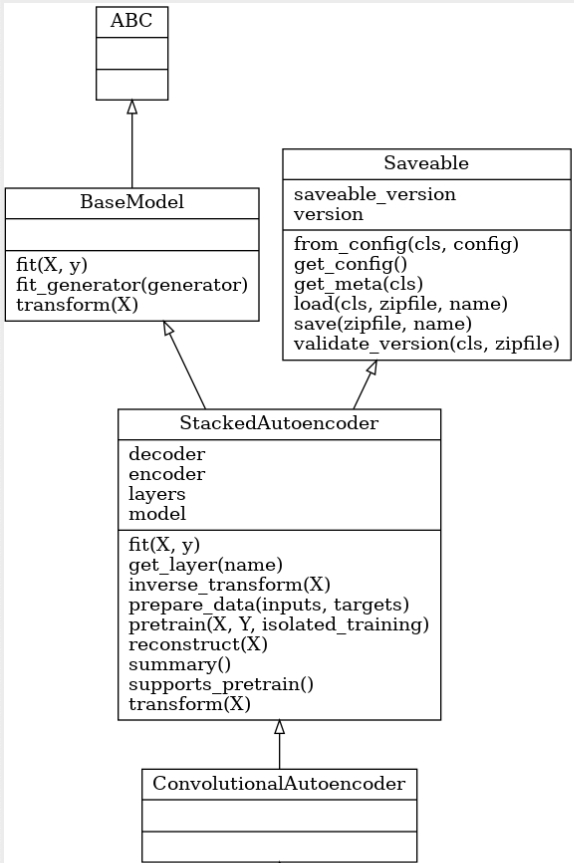
\includegraphics[width=0.5\textwidth, center]{bilder/Klassendiagramme/klassendiagramm_public_cae.png}
		\caption[Klassendiagramm ConvolutionalAutoencoder]{Klassendiagramm ConvolutionalAutoencoder}
		\label{img:KlassendiagrammConvolutionalAutoencoder}
	\end{figure}  
	
	\paragraph{hyperparameter\_mixin.py}  Hyperparameter\_mixin wird zum standardisierten Verwalten von Hyperparametern für AutoML-Klassen genutzt. Auf die Hyperaparameter kann anschließend einheitlich zugegriffen werden. Abbildung \ref{img:KlassendiagrammHyperparametermixin}  Zeigt das zugehörige UML-Klassendiagramm mit den Methoden zum Hinzufügen, Löschen und Laden der Hyperparameter. Da die Methoden öffentlich sind, können über jede erbende Klasse die Hyperparameter eigenständig verwaltet werden.
	
	\begin{figure}[h]
		\centering
		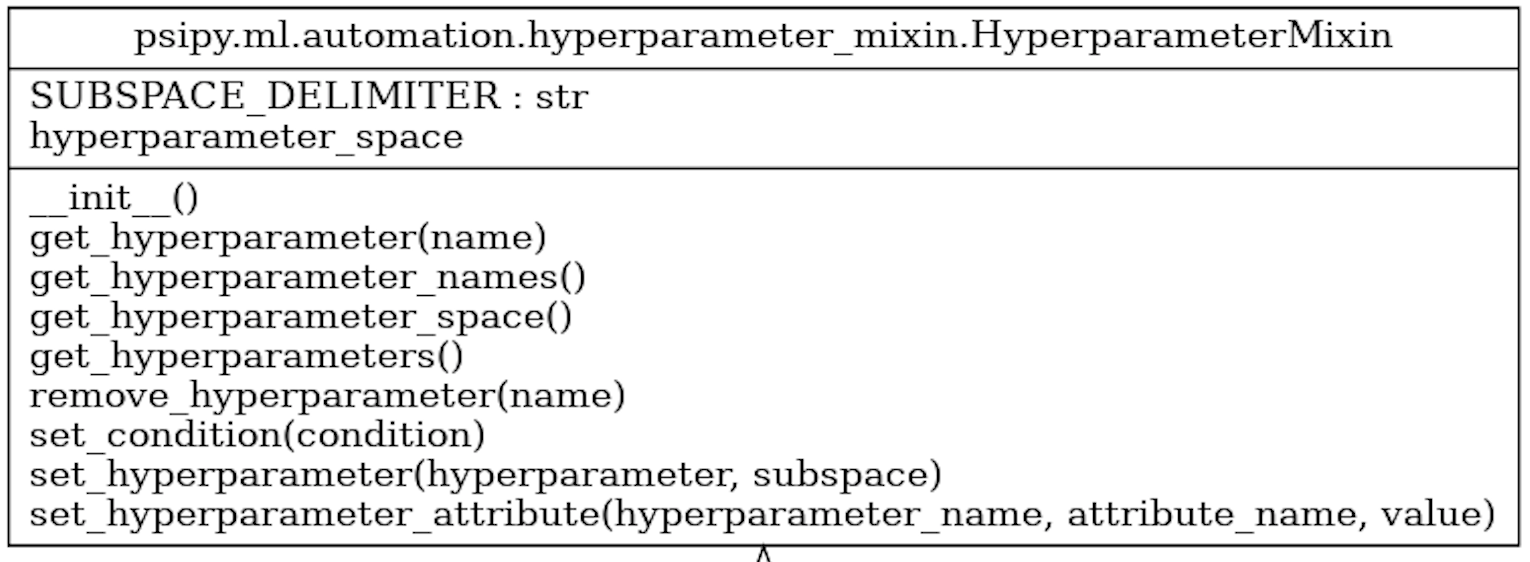
\includegraphics[width=0.5\textwidth, center]{bilder/Klassendiagramme/Hyperparametermixin.png}
		\caption[Klassendiagramm Hyperparametermixin]{Klassendiagramm Hyperparametermixin}
		\label{img:KlassendiagrammHyperparametermixin}
	\end{figure}  
	
	\section{Einordnung und bestehende Systeme}
	\label{sec:BestehendesSystem}
	Die Bilddaten und Aufgabenstellungen der neuronalen Netzwerke sind in die Problemstellungen des Autocrane-Projekts von PSIORI einzuordnen. Es sind also echte Datensätze und echte Problemstellungen, wobei die gezeigten Aufgabenstellungen und Modelle nicht zwingend in dem Autocrane-Projekt zum Einsatz kommen. Das Autocrane-Projekt ist ein laufendes Projekt, welches das Ziel hat, einen feststehenden Rundlaufkran vollautomatischen zu steuern. In Abbildung \ref{img:CircularCrane} ist ein Rundlaufkran abgebildet. Diese Art von Kran werden in holzverarbeitenden Anlagen zum Befüllen von Fülltrichtern oder Förderbändern eingesetzt. Der Kran kann sich um 360 Grad drehen. Der Greifer kann nach oben, unten und entlang mittels eines Schlittens entlang Auslegers bewegt werden. Um die Bilder aufnehmen zu können, wurde an der Kabine am Hauptstandfuß eine Kamera angebracht. Die Kamera ist auf das Ende des Auslegers und den Bereich darunter ausgerichtet. Die Kamera bewegt sich also mit dem Rundlaufkran und somit ist der Greifer immer im Bild. Für das Autocarne-Projekt sind insbesondere drei Anwendungsfälle interessant. Die Baumstämme werden mittels LKW angeliefert und müssen nach vorgegebenen Regeln (z. B. Ausrichtung, freier Lagerplatz) als Holzstapel gelagert werden. Der Fülltrichter muss mit Holz aus den Holzstapeln befüllt werden. Der Fülltrichter muss mit Holz aus einem LKW befüllt werden. Es ergeben sich also Aufgabenstellungen wie Greifer-Erkennung, Baumstamm-Erkennung, LKW-Erkennung, Strategien für das entladen und aufbewahren der Baumstämme und vieles mehr. Im Normalbetrieb werden täglich 140-200 LKW entladen. Die Ladung ist 9 - 18 Meter lang und 34 - 40 Tonnen schwer. \cite{PSIORIGmbH.2020}
	\begin{figure}[h]
		\centering
		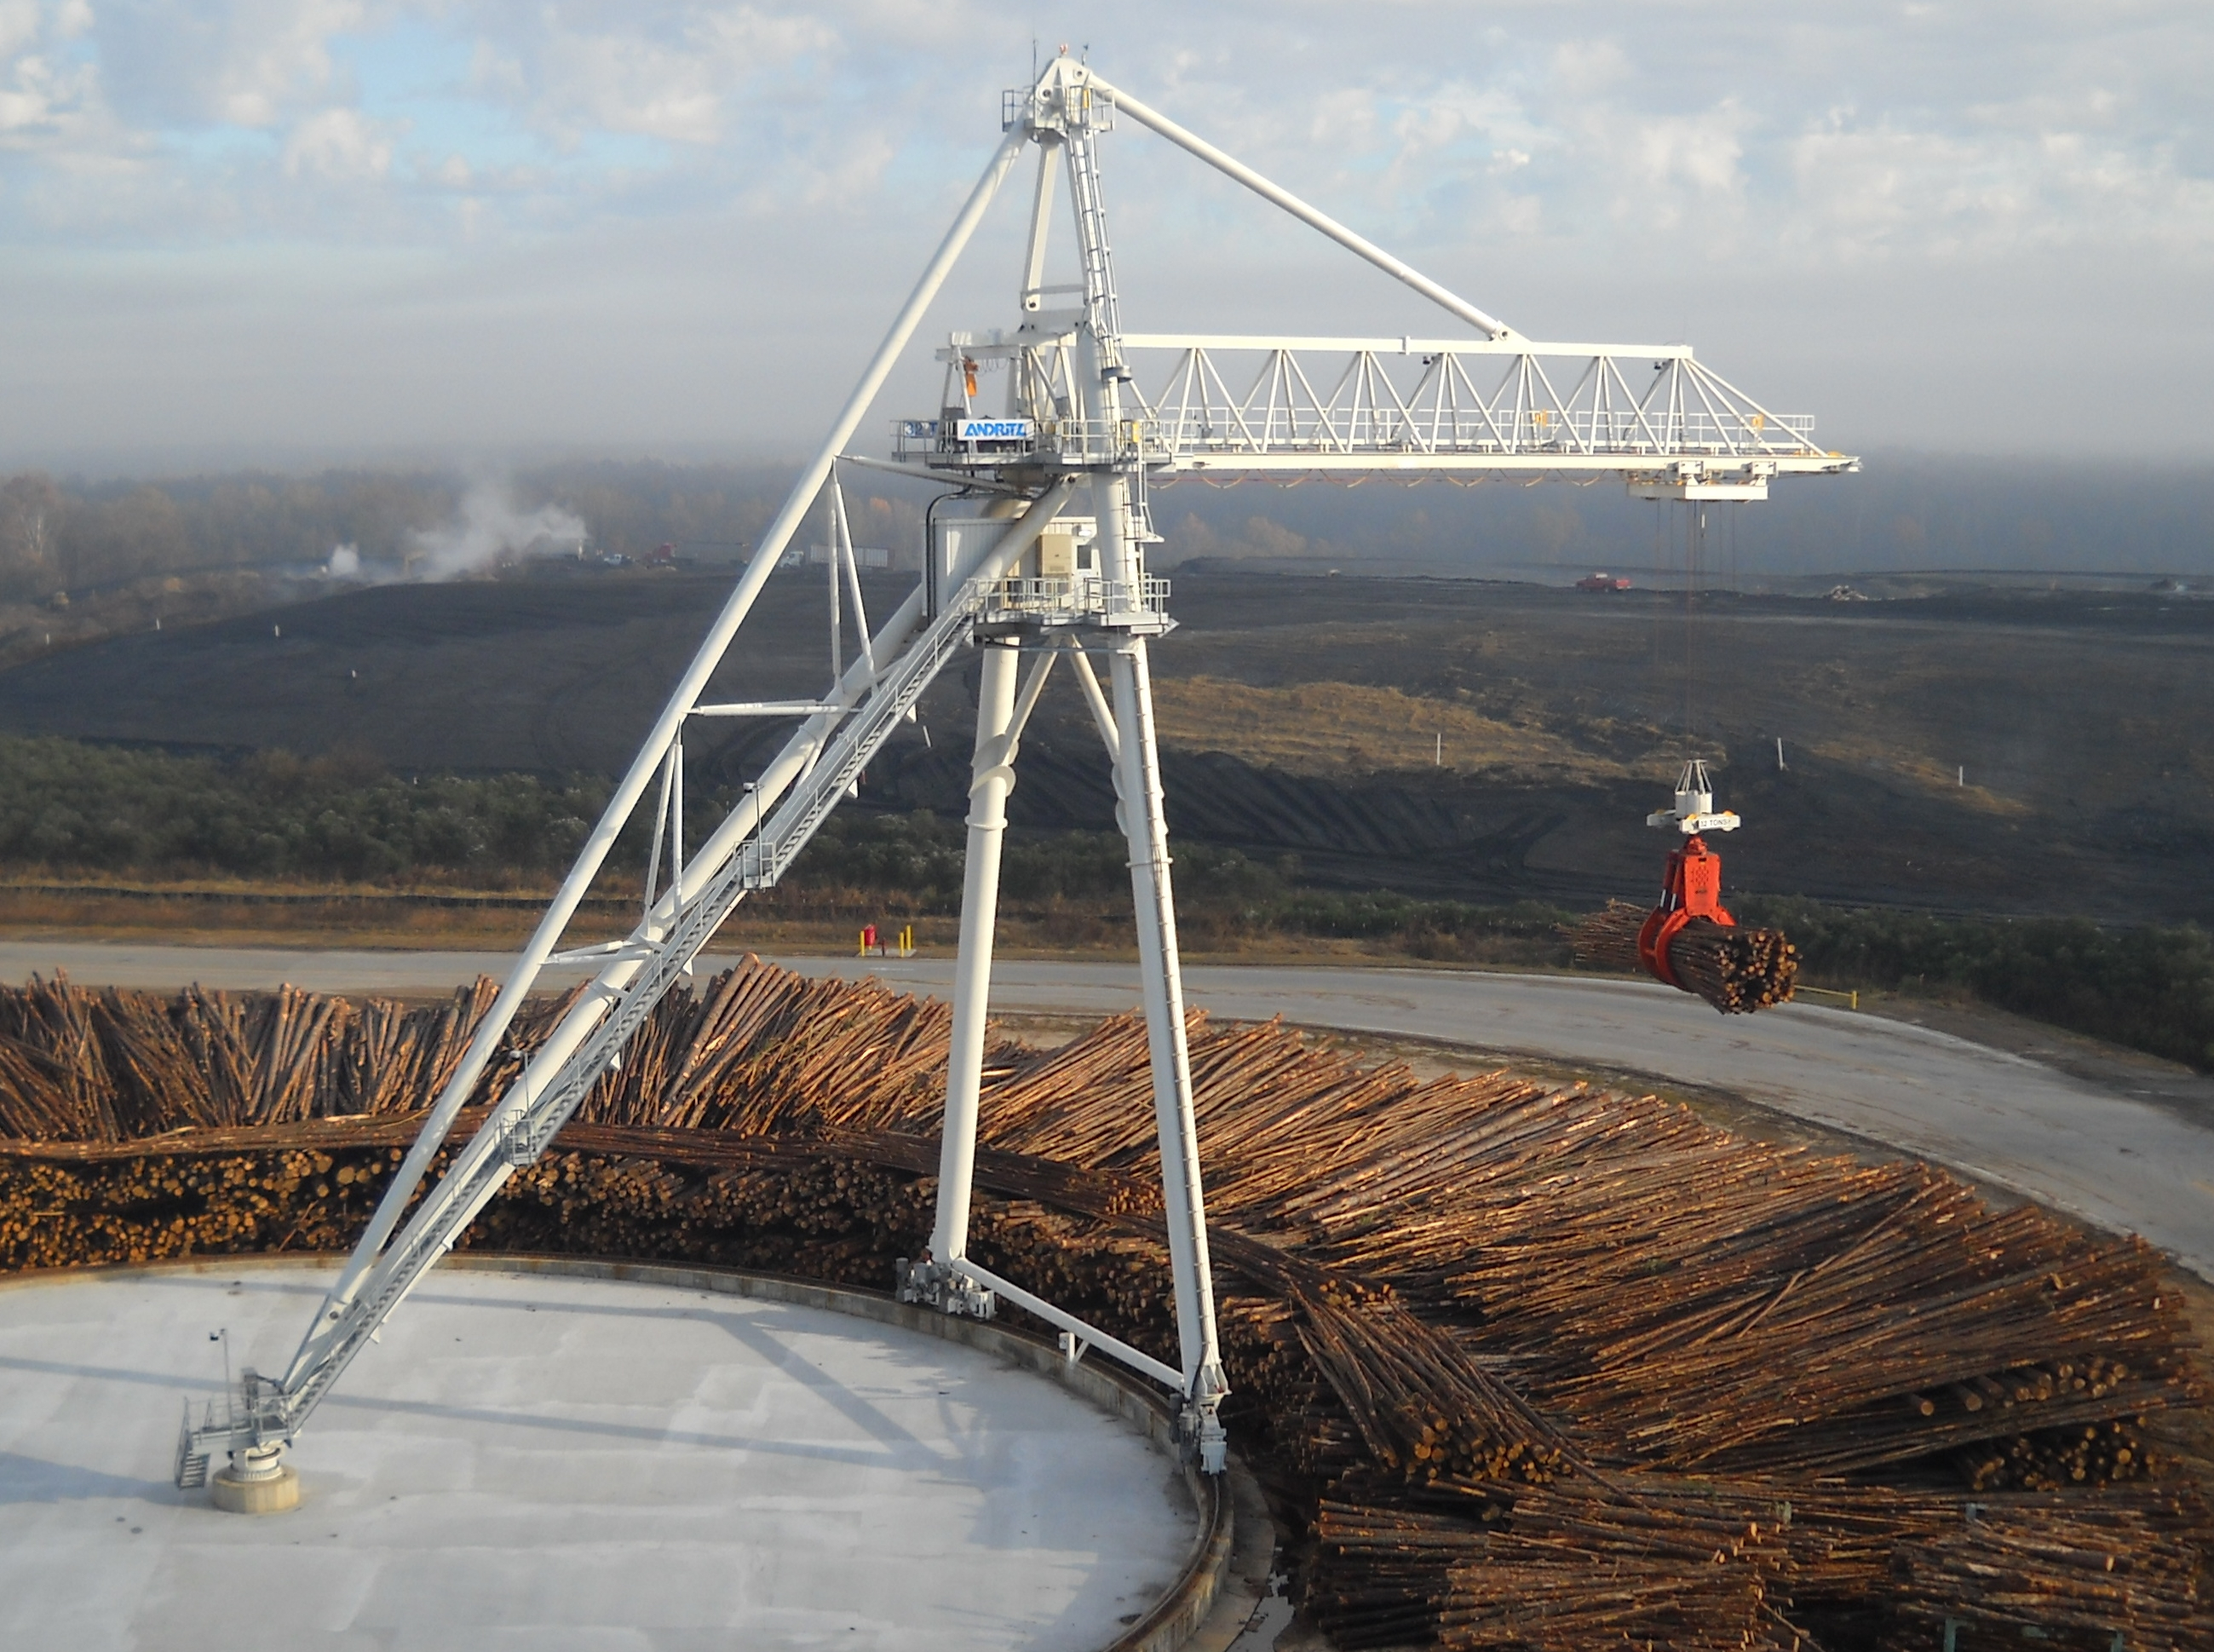
\includegraphics[width=0.5\textwidth, center]{bilder/Grundlagen/Kran_vollstaendig_N1_030.jpg}
		\caption[Rund-Kran]{Rundlaufkran (Foto: ANDRITZ)}
		\label{img:CircularCrane}
	\end{figure}		

	\paragraph{Greifererkennung} Bei der Aufgabenstellung Greifer-Erkennung muss in einem Bild die Position eines Rahmen um den Greifer gefunden werden. Abbildung \ref{img:Grapple} zeigt ein Bild mit Rahmens um den Greifer. Es handelt sich um eine klassische 'Object-Detection' Aufgabe.
		\begin{figure}[h]
		\centering
		\begin{subfigure}[c]{0.49\textwidth}			
			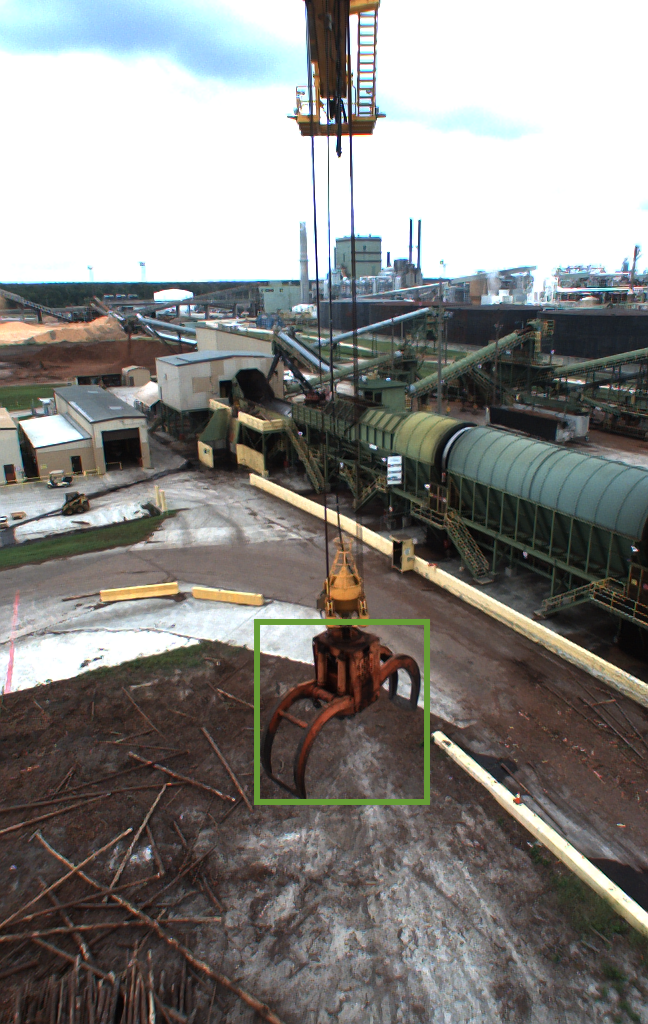
\includegraphics[width=1\textwidth, center]{bilder/Grundlagen/Grapple_8.png}
			\caption[Bsp. Bild: Greifer mit Rahmen]{Greifer mit Rahmen}
			\label{img:Grapple}	
		\end{subfigure}
		\begin{subfigure}[c]{0.49\textwidth}			
			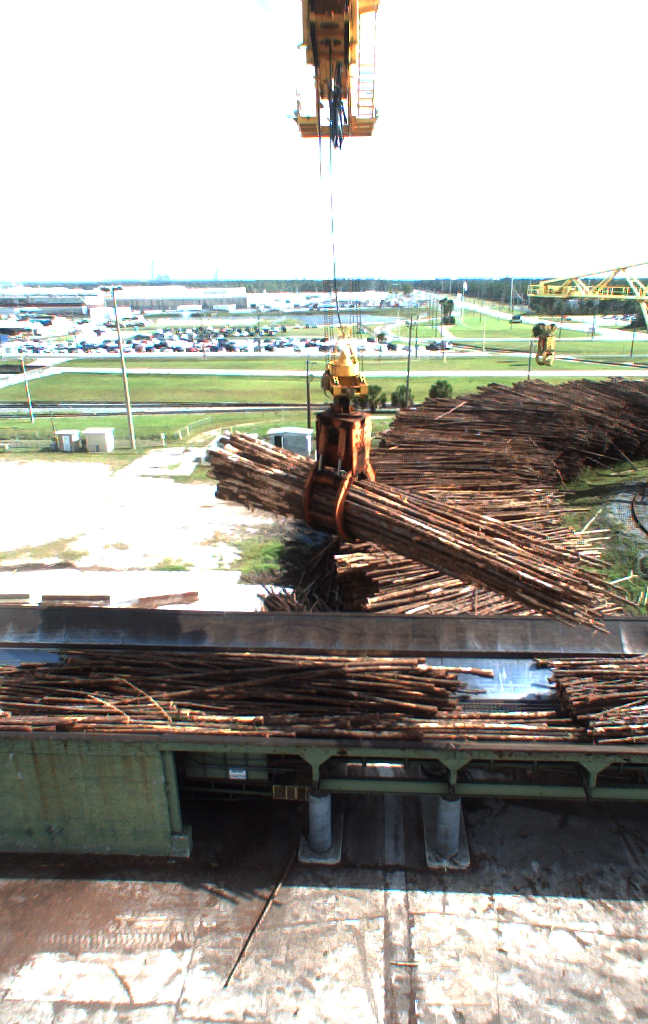
\includegraphics[width=1\textwidth, center]{bilder/Grundlagen/Logs_14.png}
			\caption[Bsp. Bild: Greifer mit Baumstämmen]{Greifer mit Baumstämmen}
			\label{img:Logs}	
		\end{subfigure}
		\caption{Greifer}
		\label{img:Greifer}
	\end{figure}	

	PSIORI hat die Aufgabe mittels neuronalem Netzwerk gelöst. Dabei wurde auf die Technik des Single Shot MultiBox Detector (SSD) [todo https://arxiv.org/abs/1512.02325] zurückgegriffen. Das Netz liegt als frozen\_inference\_graph.pb vor. Protocoll Buffer  [https://developers.google.com/protocol-buffers/] ist ein sprachneutraler, plattformneutraler, erweiterbarer Mechanismus zur Serialisierung strukturierter Daten. In diesem Fall enthält die Datei den eingefrorenen Graph und die Model Gewichte. Um Vorhersagen treffen zu können, wurde eine Klasse erstellt, welche mittels einer Tensorflowsession und dem Model vorhersagen trifft.  abei liefert das Model pro Bild einen Rahmen, in welchem sich der Greifer befindet und einen Vertrauenswert. Der Vertrauenswert sagt aus, wie sicher sich das Netzt mit seiner Aussage ist. Die Vorhersagegenauigkeit dieses Modells wird als Basislinie und Vergleichswert für die durchgeführten Versuche genutzt.
		
	\paragraph{Baumstammklassifikation} Die Aufgabe der Baumstammklassifikation hat zum Ziel, zu erkennen ob sich Baumstämme im Greifer befindet oder nicht. Es handelt sich um eine Klassifikationsaufgabe.
	Ein Klassifikatior, für die Frage ob sich Baumstämme in dem Greifer befinden liegt als Tensorflow-MetaGraph[https://www.tensorflow.org/api\_docs/python/tf/compat/v1/train/import\_meta\_graph] vor. Um Vorhersagen treffen zu können, wurde eine Klasse,welche den MetaGraph nutzt erstellt. Die Vorhersage des Modells liefert die vorhergesagte Klasse mit einer Wahrscheinlichkeit zurück. Dieses Model wird wie das Greifererkennung Model als Basislinie und Vergleichswert für die durchgeführten Versuche genutzt.

	\section{Datenverständnis}
	\label{sec:DataUnderstanding}
	Mittels Kamera an der Kabine können neue unbeschriftete Bilder aufgenommen und bei PSIORI abgelegt werden. Durch den Aufbau des Rundkrans und der Kameraposition befindet sich der Greifer immer im Bild. Der Hintergrund der Bilder ändert sich stark. Die geografische Lage des Rundkrans ist im Hinblick auf das Wetter positiv. Es fällt kein Schnee und es gibt wenige Regentage. In Abbildung  \ref{img:Bildqualität} sind Ausprägungen der Bildqualität dargestellt. Abgesehen von Bildern in guter Qualität gibt es helle Bilder, dunkle Bilder und Bilder mit Reflexionen. Die Bilder sind 1024 auf 648 Pixel groß und in Farbe. Die einzelnen Pixel können dabei Werte zwischen 0 und 255 annehmen. 
	Entsprechend der beiden Aufgabenstellungen Greifererkennung und Baumstammklassifikation werden Daten mit einer passenden Beschriftung benötigt.
	
	\begin{figure}[h]
		\centering
		\begin{subfigure}[c]{0.24\textwidth}			
			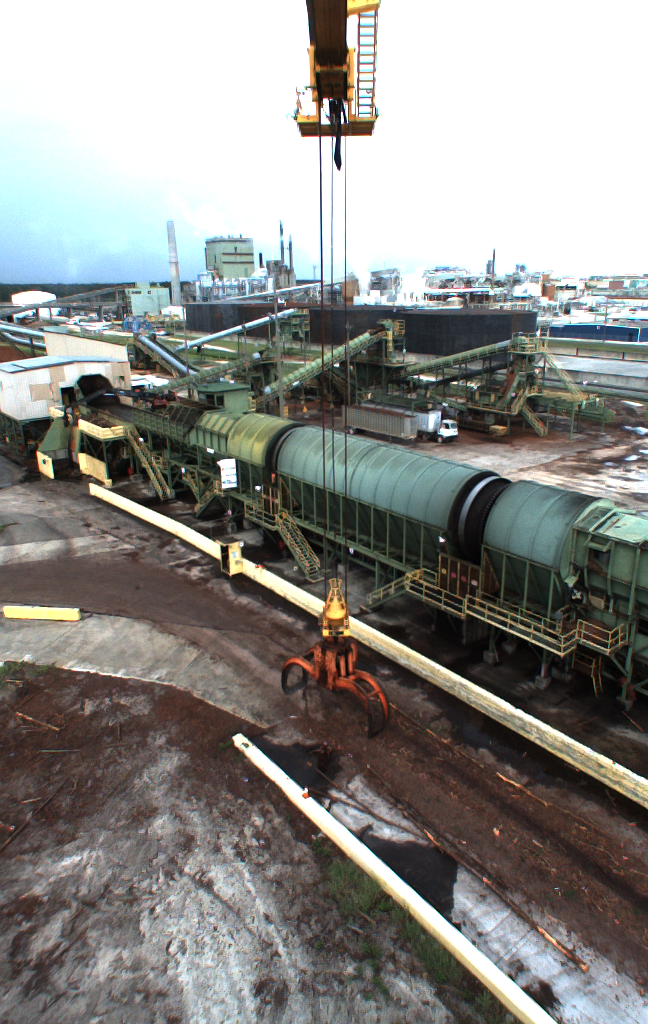
\includegraphics[width=1\textwidth]{bilder/Grundlagen/Daten_Bildqualitaet/gut.png}
			\subcaption{Gut}			
		\end{subfigure}
		\begin{subfigure}[c]{0.24\textwidth}			
			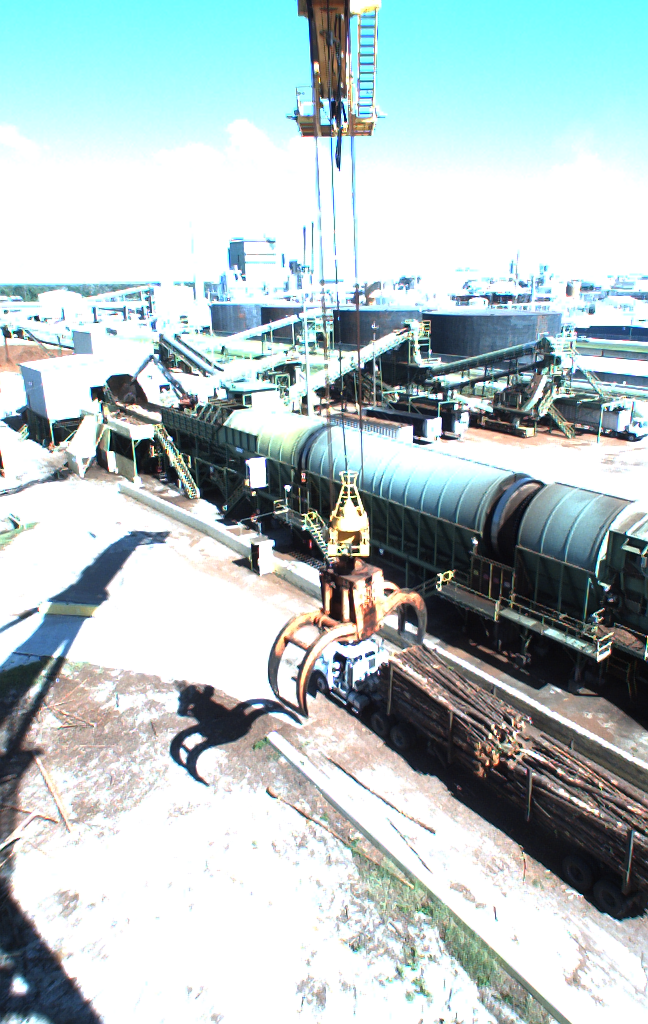
\includegraphics[width=1\textwidth]{bilder/Grundlagen/Daten_Bildqualitaet/hell.png}
			\subcaption{Hell}			
		\end{subfigure}
		\begin{subfigure}[c]{0.24\textwidth}			
			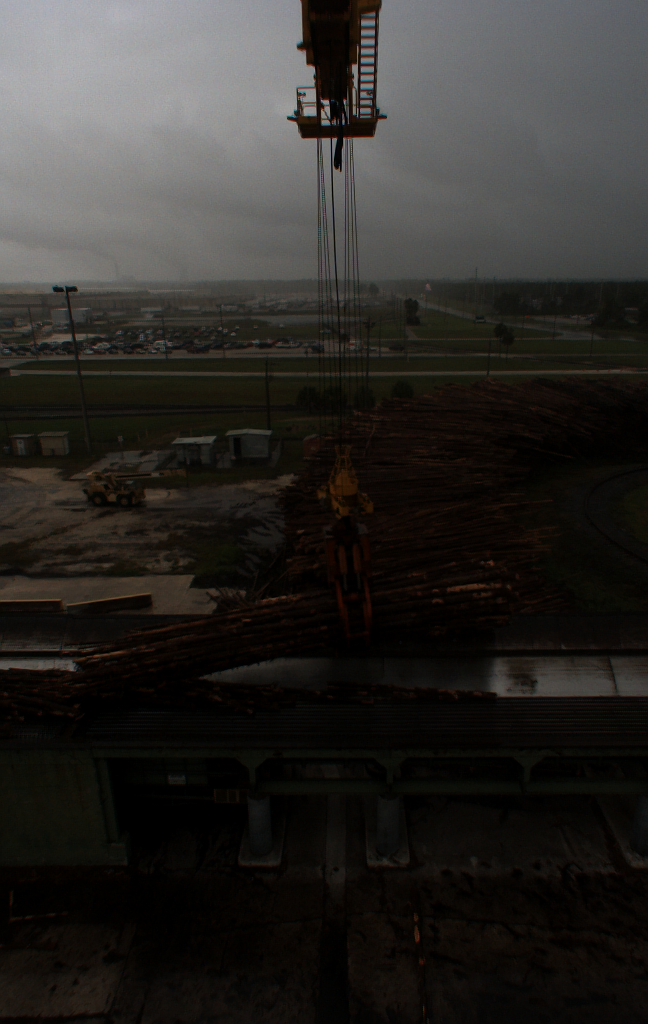
\includegraphics[width=1\textwidth]{bilder/Grundlagen/Daten_Bildqualitaet/dunkel.png}
			\subcaption{Dunkel}			
		\end{subfigure}
		\begin{subfigure}[c]{0.24\textwidth}			
			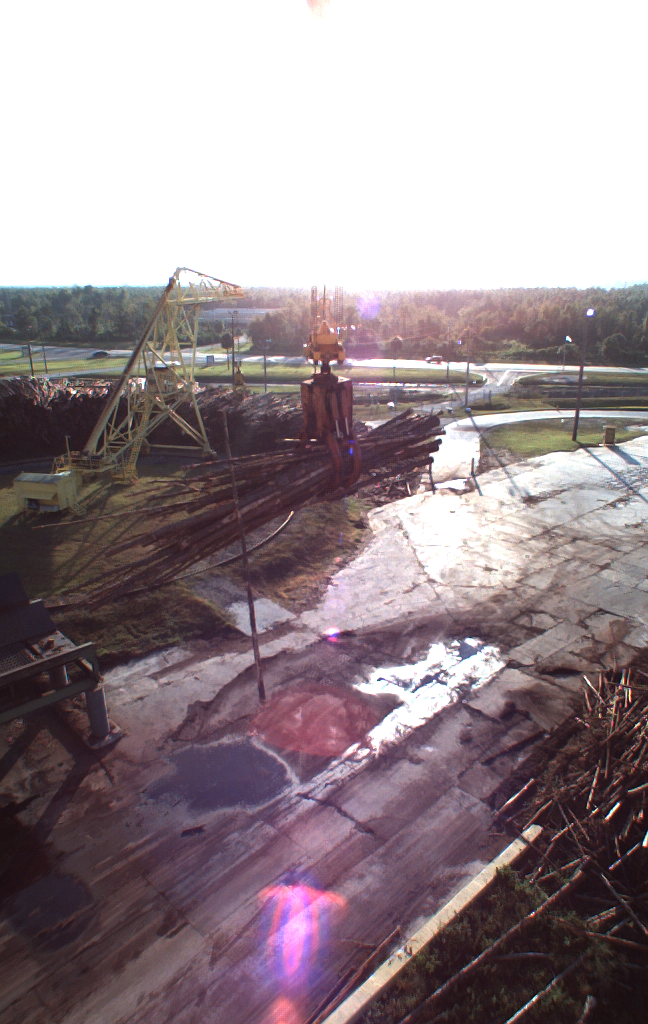
\includegraphics[width=1\textwidth]{bilder/Grundlagen/Daten_Bildqualitaet/Reflexionen.png}
			\subcaption{Reflexionen}			
		\end{subfigure}
		\caption{Bildqualität}
		\label{img:Bildqualität}
	\end{figure}
		
	\paragraph{Greiferdatensatz} Der Greifer Datensatz enthält Bilder, in welchen der Greifer mittels Rahmen markiert ist. Abbildung \ref{img:Grapple} zeigt ein beispielhaftes Bild mit markiertem Greifer. Die Annotationen der Position des Greifers wurde pro Bild in einer XML-Datei abgelegt. Konkret wurde die Position als x, y Koordinaten in der Form ymin, xmin, ymax und xmax  abgespeichert. Über die vier Werte lässt sich problemlos ein Rahmen um den Greifer spannen. Der Datensatz besteht aus 4.684 durch Personen annotierten Bildern.
	 
	\paragraph{Baumstammdatensatz} Der Baumstamm Datensatz enthält Bilder, welche die Annotation, ob sich Baumstämme im Greifer befinden oder nicht enthält. Die Bilder sind durch zwei Ordner in Bilder mit und Bilder ohne Baumstämme aufgeteilt. Abbildung \ref{img:Logs} zeigt ein Bild, in welchem der Greifer Baumstämme greift. In Abbildung \ref{img:Grapple} befinden sich keine Baumstämme im Greifer.
	Im Gegensatz zu dem Greiferdatensatz wurde dieser Datensatz (zum Teil) im Rahmen der Abschlussarbeit angefertigt. Hierzu wurde mit Quality Match GmbH [https://www.quality-match.com] zusammengearbeitet. Die Quality Match GmbH arbeitet mit Crowdworkern zusammen, um Datensätze mit kontrollierter Annotationsqualität zu erstellen.  

	\paragraph{Weiterer Datensatz} Für Mitte 2020 ist ein weiterer Datensatz geplant. Dieser Datensatz enthält circa 80.000 beschriftete Bilder. Er wird sowohl die Annotation 'Logs ja / nein' als auch die Rahmen um den Greifer enthalten. Zusätzlich sind für diesen Datensatz weitere Beschriftungen wie Helligkeit, Winkel des Greifers und weitere Annotationen geplant. 
			
	\section{Datenvorbereitung}
	\label{sec:DataPreparation}
	In Vorbereitung auf die Modellierungsphase wurde ein finaler Datensatz erstellt und Werkzeuge zum Laden und vorbereiten der Daten implementiert.
	\paragraph{Erste Iteration} Als Erstes wurden die Daten mittels Skripten in Training, Test und Validation Daten aufgeteilt. Anschließend wurden die Daten auf der Cnvrg-Plattform in einen versionierbarer Datenspeicher geladen. In Tabelle \ref{table:DatenaufteilungTrainTestValidation} ist die finale Datenaufteilung zu sehen. Die Greifer Daten sind in 70\% Trainingsdaten und jeweils 15\% Test und Validierungsdaten aufgeteilt. Die Baumstammdaten sind in 80\% Trainingsdaten 10\% Testdaten und 10\% Validierungsdaten getrennt worden. Die Trainingsdaten werden zum Trainieren der Modelle genutzt, die Testdaten zum Überprüfen der Modelle und die Validierungsdaten werden am Ende der Experimente als finale Überprüfung der Ergebnisse eingesetzt.
	\begin{table}[ht]
		\centering
		\begin{tabularx}{\textwidth}{lllll}
			& \textbf{Train} & \textbf{Test}  & \textbf{Validation} & \textbf{Summe} 	 \\
			\textbf{Greifer} 				 & 	3.279			& 703	 & 704				   & 4.686 	\\
			\textbf{Baumstämme j/n}	 	  &  9.749	   & 1.221 	& 1.225	& 12.195\\		
		\end{tabularx}
		\caption{Datenaufteilung - Train Test Validation}
		\label{table:DatenaufteilungTrainTestValidation}
	\end{table}
	
	Für das Laden der Daten wurde ein Modul 'data\_loader.py' erstellt. Dieses Modul enthält die drei Klassen DataLoader, GrappleDataLoader, LogsDataLoader. DataLoader ist eine abstrakte Klasse, welche Methoden zum Laden der Train-, Test- und Validationdaten definiert. Sie liefern entsprechend eines Parameters, bis zur maximalen Anzahl an Bildern, Bilder als Numparray zurück. Die Klassen GrappleDataLoader und LogsDataLoader implementieren für den jeweiligen Datensatz die konkreten Methoden zum Laden der Daten.
	
	Mittels dem Modul 'data\_preparation.py' und der Klasse Preprocessing werden die Bilder auf die passende Größe verkleinert oder vergrößert und auf den Wertebereich zwischen 0 und 1 normalisiert.
	
	\paragraph{Zweite Iteration} 
	In der zweiten Iteration wurde ein neues Modul namens data\_generator\_provider.py erstellt. Da Bilder als Numpyarray direkt in den Speicher geladen werden können nicht beliebig viele Bilder genutzt werden. Dieses Problem wird von den Keras ImageDataGeneratoren [https://keras.io/preprocessing/image/] adressiert. Sie erlauben es Bilder stapelweise bereitzustellen. Zusätzlich werden bei den Imagedatageneratoren direkt die Zielgrößen bereitgestellt. Das Modul implementiert jeweils für den Baumstamm Datensatz und den Greiferdatensatz eine Klasse zum Bereitstellen von ImageDatageneratoren.
	
	Da die Modelle Mehrfach-Ausgang-Modelle sind erfolgt zusätzlich noch eine Aufbereitung der Bereitstellung der Daten. Standardmäßig stellen die Generatoren Stapel mit Einträgen der Form $X ,Y$  bereit. Wobei X die Eingangsdaten sind und Y die Zielgröße. Zum Beispiel kann X ein Bild sein und Y die zugehörige Klasse. Die Werkzeuge mit zweitem Kriterium benötigen Generatoren die Einträge der Stapel der Form $X, [X, Y]$ erzeugen. Die Zielgröße hat sich zu einer Liste mit zwei Größen verändert. Die erste Zielgröße entspricht den Eingangsdaten, sie werden für den Decoder-Ausgang genutzt. Die zweite Zielgröße wird für den zweiten Ausgang genutzt. Sie entspricht der Zielgröße eines normalen ImageDataGeneratoren. Das Ganze wird mit Hilfe der Klasse tensorflow.keras.utils.Sequence erreicht. Ihr wird im Konstruktor ein ImageDataGenerator übergeben. Bei der Bereitstellung eines Elementes wird der Rückgabewert des Generators angepasst. Die entscheidenden Codezeilen sind in Listing \ref{lst:AufbereritungGeneratorergebnis} dargestellt. 
	\begin{lstlisting}[language=python,caption=Aufbereitung Generatorergebnis in Python, label=lst:AufbereritungGeneratorergebnis]
		res = self.generator.next()
		return res[0], [res[0], res[1]]
	\end{lstlisting}
	
	Für das Vortrainieren werden Generatoren bereitgestellt, welche Stapel mit Einträgen der Form $X ,X$ erzeugen. Hierbei wird auf Standardfunktionalität der Klasse ImageDataGenerator zurückgegriffen.
	
	Die ImageDataGeneratoren bieten Standardfunktionalität zum Anpassen der Daten. Alle Generatoren normalisieren die Werte der Bilder zwischen 0 und 1. Die Generatoren für die Trainingsdaten führen noch zufällige Veränderungen der Helligkeit und Kanalverschiebungen durch. Bei den Baumstamm Daten werden die Bilder zusätzlich horizontal umgedreht. 


 


 
